\documentclass[12pt,a4paper,titlepage,spanish]{article} 
\usepackage{babel}
\usepackage [T1]{fontenc}
\usepackage [latin1]{inputenc}
\usepackage{graphicx}
\usepackage{amssymb}
\usepackage{amsmath}
\usepackage{setspace}
\usepackage{epsfig}
\usepackage{enumerate}
\usepackage{float}
\usepackage{array}
\usepackage{cancel}
%\usepackage{arcs}
\usepackage[usenames,dvipsnames]{color}

	  \oddsidemargin 0in
      \textwidth 6.75in
      \topmargin 0in
      \textheight 10.0in
      \parindent 0em
      \parskip 2ex
\usepackage{anysize}
\marginsize{3cm}{2cm}{1.0cm}{1.0cm}
\pagestyle{plain}
\title{
\begin{Large}
 \begin{center}
		\underline{Informe simulaciones TP07 - M�todo de Montecarlo}\\
		\underline{Curso: } 6to 1ra\\
		\underline{Turno: } Noche\\
		\underline{CPU: } Intel Core 2 Duo E6600\\
      \end{center}
\end{Large}
}
\author{Vileri�o, Silvio}

\begin{document}
\maketitle
\setcounter{page}{2}
\tableofcontents
\newpage

\subsection{Introducci�n}
Esta simulaci�n se desarrolla con el fin de comprobar la calidad del generador de numeros aleatorios (GNA) basado en la teoria del c�os num�rico.\\
Su f�rmula es: $ X = \{ k \times X  \}$\\
Donde $ \{ \} $ es la mantisa o parte decimal.\\
El valor calibrado de K es $ K=2555 $. El generador presenta buenos resultados con n�meros $ k $ impares de gran magnitud. $ k=2n+1 $ con $ n>1200 $ aproximadamente.
La semilla inicial se calcula con la funcion GNA de Java.
\newpage
\subsection{An�lisis}
Al GNA se le realizan las siguientes pruebas:\\
\begin{itemize}
	\item Se calcula un promedio $ \bar X $ de 1000000 n�meros generados al azar.\\
		$ \bar X = \frac{\displaystyle{\sum_{k=1}^n} {a_k}}{n}, n=1000000 $
	\item Se calcula la dispersi�n $ \sigma^2 $ entre cada n�mero generado y el promedio obtenido anteriormente.\\
		$ \sigma^2 = \frac{\displaystyle{\sum_{i=1}^n {(X_i - \bar X)^2}}}{n}, n=1000000, \bar X \longrightarrow $ promedio
	\item Se confecciona un histograma donde se registran la cantidad de n�meros generados entre 0,0 exclusive y 0,1 exclusive, en 10 intervalos de 0,1
	\item Se calcula $ \bar f $, la frecuencia promedio de los intervalos.\\
	$ \bar f=\frac{\displaystyle{\sum_{i=1}^n {k_i}}}{n},n=10, k_i \longrightarrow $ frecuencia registrada en cada intervalo.
	\item Se calcula la dispersion $ \sigma^2_{hist} $ entre las frecuencias del histograma y la frecuencia promedio obtenida anteriormente\\
	 $ \sigma^2_{hist}=\frac{\displaystyle{\sum_{i=1}^n {(F_i - \bar f)^2}}}{n}, n=10 $
	 \item Se realizan dos pruebas gr�ficas en las que se generan 250000 puntos al azar en un �rea de $ 500 \times 500 $ p�xeles. \begin{itemize}
	 											\item Paralelo: se toman dos GNA con distinta semilla , para x e y .
	 											\item Serie: se toman dos GNA y se mantiene esta relaci�n para la generaci�n de valores de x e y :$ x=GNA(GNA(x)) $, previamente x siendo la semilla inicial.
	 												 			
	 										\end{itemize}
	 \item Se busca el per�odo del GNA.
\end{itemize}
\newpage
\subsection{Resultados Anal�ticos}
Luego de realizar la simulaci�n, se obtuvieron los siguientes resultados: \\

\begin{itemize}
		\item Promedio $ \longrightarrow  \bar X = 0.5004766434926292 $ 
		 \item Dispersi�n $ \longrightarrow \sigma^2 = 0.08327092587874708 $  
		\item Histograma: \begin{itemize}	
			\item Intervalo $ \left( 0.0 ; 0.1 \right)= 99764 $
			\item Intervalo $ \left[ 0.1 ; 0.2 \right)= 99621 $
			\item Intervalo $ \left[ 0.2 ; 0.3 \right)= 99562 $
			\item Intervalo $ \left[ 0.3 ; 0.4 \right)= 100205 $
			\item Intervalo $ \left[ 0.4 ; 0.5 \right)= 100448 $
			\item Intervalo $ \left[ 0.5 ; 0.6 \right)= 100036 $
			\item Intervalo $ \left[ 0.6 ; 0.7 \right)= 99916 $
			\item Intervalo $ \left[ 0.7 ; 0.8 \right)= 99968 $
			\item Intervalo $ \left[ 0.8 ; 0.9 \right)= 100260 $
			\item Intervalo $ \left[0.9 ; 1.0 \right)= 100220 $
		\end{itemize}
\item Frecuencia Promedio $ \longrightarrow \bar f = 100000 $
\item Dispersi�n del Histograma $ \longrightarrow \sigma^2_{freq. hist.} = 75928.6 $
\item Periodo: 946446
\end{itemize}
\newpage

\subsection{Resultados Gr�ficos}
\underline{Histograma}\\
\begin{center}
	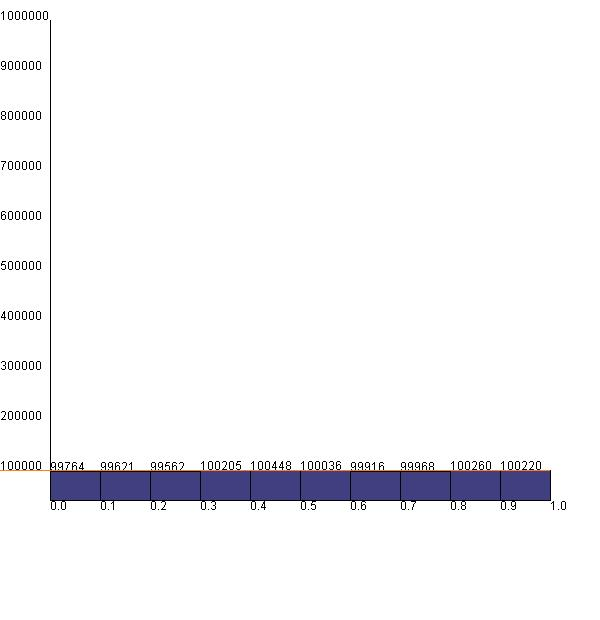
\includegraphics[scale=0.75]{images/Histograma.jpg}
\end{center}
\newpage
\underline{Test Gr�fico Paralelo}
\begin{center}
	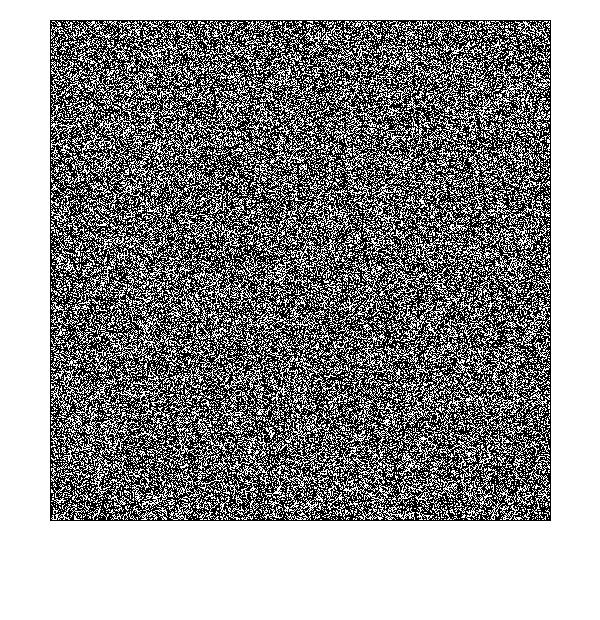
\includegraphics[scale=0.75]{images/Paralelo.jpg}
\end{center}
\newpage
\underline{Test Gr�fico Serie}
\begin{center}
	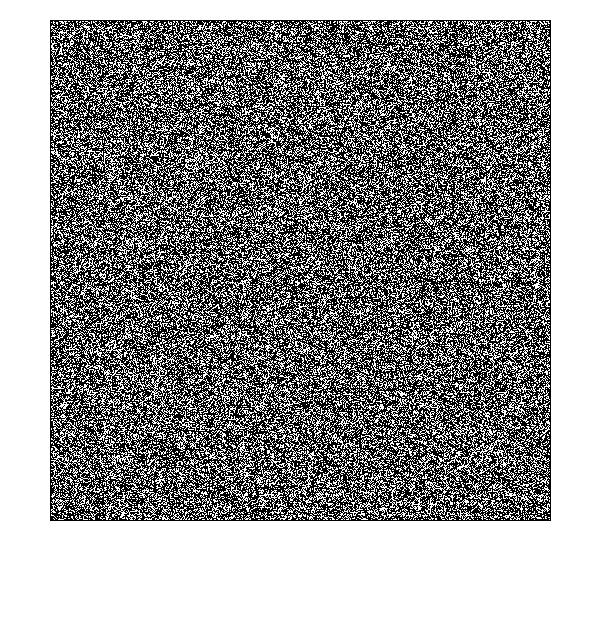
\includegraphics[scale=0.75]{images/Serie.jpg}
\end{center}
\newpage
\subsection{Conclusi�n}
Se infiere de los resultados obtenidos que el GNA es bueno, ya que el promedio, $ \bar X \simeq \frac{1}{2} $, la dispersi�n $ \sigma^2 \simeq 0.08 \dots $, y las pruebas gr�ficas, junto con el histograma y su dispersi�n cumplen con las condiciones establecidas de un buen GNA. Con valores $ k $ impares peque�os, los per�odos se hacen mas peque�os, es decir, se repiten m�s n�meros, por eso es muy importante utilizar valores correctamente calibrados y testeados.
\end{document}